\documentclass[11pt,a4paper]{article}
\title{APG4011F Assignment 2 Report}
\date{21 April 2015}
\author{Tim Marsh}

\usepackage{amsmath}
\usepackage{graphicx}
\usepackage{float}
\usepackage{textcomp}
\usepackage{siunitx}
\usepackage{wrapfig}
\usepackage{caption}
\usepackage{subcaption}

\usepackage[margin=1in]{geometry}

\graphicspath{ {./} }
\begin{document}
	
	\pagenumbering{gobble}
	\maketitle
	\begin{figure}[H]
		\centering
		
\includegraphics[width=0.7\linewidth]{./UCTcircular_logo1_CMYK}
		\label{fig:UCTcircular_logo1_CMYK}
	\end{figure}
	\newpage
	\pagenumbering{arabic}
	\tableofcontents
	\listoffigures
	\newpage
	
	
	\section{Introduction}
	
	This aim of this assignment was to write a program that classifies a points cloud based on weather that point belongs to the floor(normal pointed up) or the wall(normal pointed at 90\si{\degree} to vertical).
	
	To do this a normal for each point is calculated then the angle between that points normal and the vertical vector $[0,0,1]$, is used to classify the point. 

	\section{Background to the Problem}
	
	To do this assignment a program that reads a large point cloud in and preforms actions on each point is required. The issue with writing programs that work with big data is that they tend to be slow. Python 3.4 was used in this assignment. The standard for working with large data such as point clouds is to use C++ because it is significantly faster.
	
	It is however harder to understand and to code and in such a short time frame it is easier to deal with python being slower.
	
	Using Python isn't the end of the world thought because there are many ways to make it faster. the first and easiest to implement is using \textit{cKDTree} over \textit{KDTree}. The only major difference between these two is that \textit{cKDTree} is a C++ module being used in a python program. After a quick test it is evident that \textit{cKDTree} runs about 10 times faster that \textit{KDTree}.
	
	\begin{wrapfigure}{l}{0.5\textwidth}
		\centering
	 	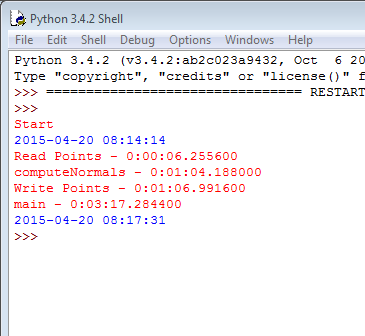
\includegraphics[width=0.8\linewidth]{./consoloutput}
	 	\caption{Console Output}
	 	\label{fig:consoloutput}
	\end{wrapfigure}
		
	Another way to significantly speed up running large data sets in python is to use a package called Multiprocessing, using the Pool object which offers an easy way of parallelizing the execution of a function across multiple input values.

	This helped speed up the program by allowing 4 quadrants of the scan to be processed independently (4 because there ar 4 cores in the computer it was run on).
	
	This took the normal computation function from taking around 8 minutes to run 2.2 million down to 2 minutes.
	
	Before all these time saving features were implemented the code took around 13 minutes to run, now it takes 3 minutes.
	
	\newpage
	\section{Method}
	
	The method followed in this assignment is as follows:
	
	\begin{enumerate}
	\item Read a point cloud file in .xyz format
	
	\item Calculate a KDTree for the point cloud
	
	\item Then for a point use the KDTree to find the nearest K neighbours.
	
	\item Then using a Principal Components Analysis calculate the normal to the set neighbours of the point.
	
	\item Save that normal vector and calculate the angle between the normal and the vertical vector $[0,0,1]$ then save that angle with the point as well.
	
	\item Then classify the point based on the angle it has from the vertical. There were 3 classes in this program:
	
	\begin{description}
	 \item[As class 1] between 0\si{\degree} and 40\si{\degree} from the vertical
	 \item[As class 2] between 40\si{\degree} and 60\si{\degree} from the vertical
	 \item[As class 3] between 60\si{\degree} and 90\si{\degree} from the vertical
	\end{description}
	
	The angles are all normalised between 0\si{\degree} and 90\si{\degree}.
	
	\item Repeat steps 3 to 6 for every point in the point cloud.
	
	\item Finally write the points with their normals and angles to a new file
	
	\end{enumerate}
	
	Once the program has run and saved everything the point cloud (in a .xyz format) is moved into cloud compare.
	
	\section{Results}
	What became apparent early on in that the value of K is very important. The value of K corresponds with how many other points you choose from the neighbourhood around each point.
	
	The best values for K were found to be 20, 40 and 60.
	
	\begin{minipage}{0.9\textwidth}
	\begin{minipage}{.5\textwidth}
		
		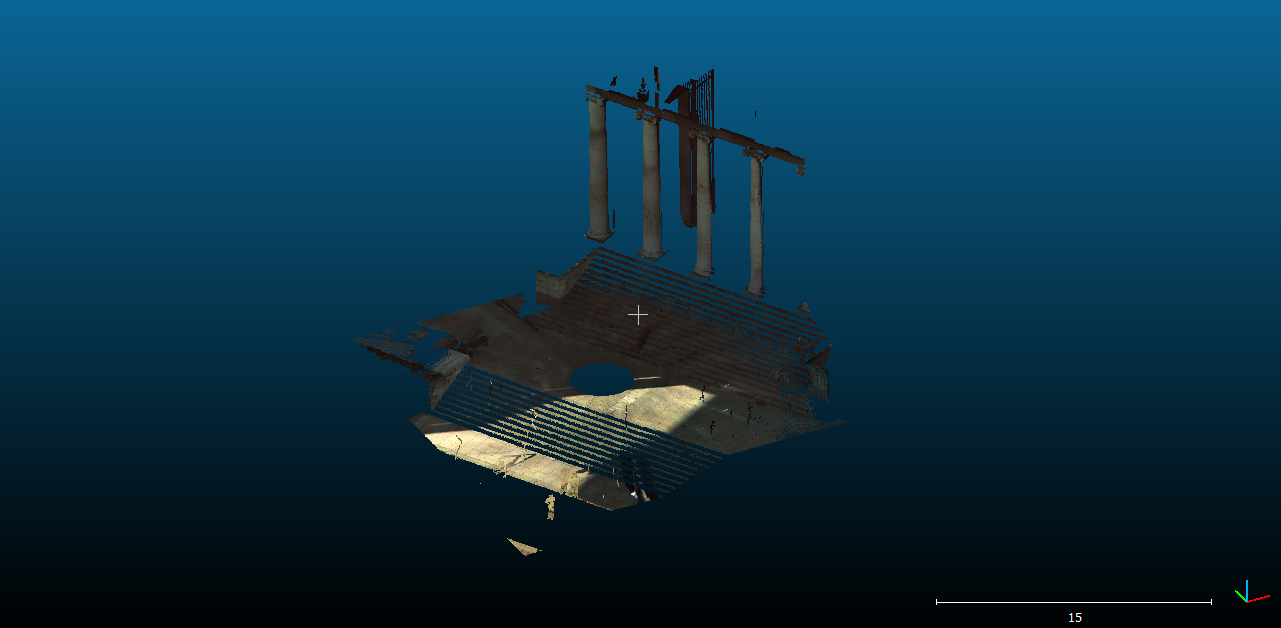
\includegraphics[width=0.8\linewidth]{./Before}
		\captionof{figure}{{\footnotesize Original Scan}}
		\label{fig:Before}

	\end{minipage}%
	\begin{minipage}{.5\textwidth}
		
		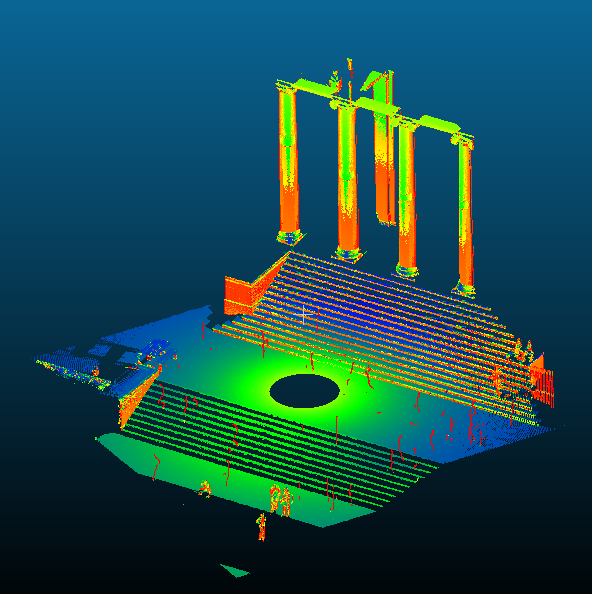
\includegraphics[width=0.8\linewidth]{./Anglek=20}
		\captionof{figure}{{\footnotesize Angle from
		vertical with $K = 20$}}
		\label{fig:Angleformvertk=20}
	\end{minipage}
	
	\begin{minipage}{.5\textwidth}
		
		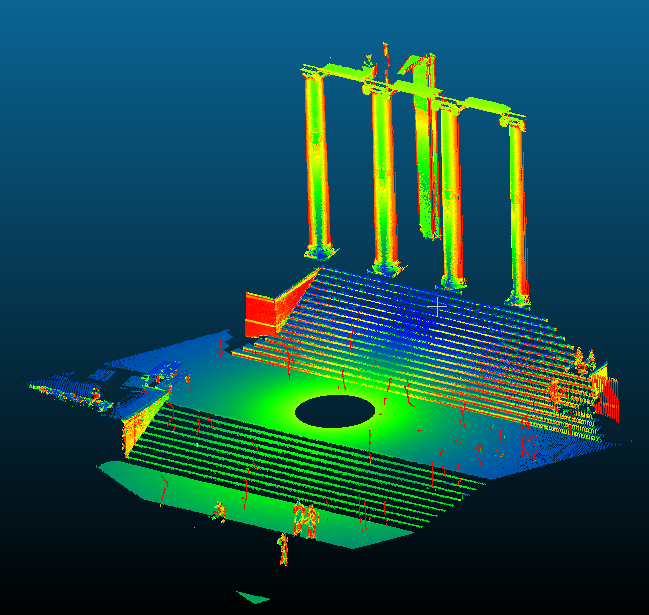
\includegraphics[width=0.8\linewidth]{./Anglek=40}
		\captionof{figure}{{\footnotesize Angle from
		vertical with $K = 40$}}
		\label{fig:Angleformvertk=40}
	\end{minipage}%
	\begin{minipage}{.5\textwidth}
		
		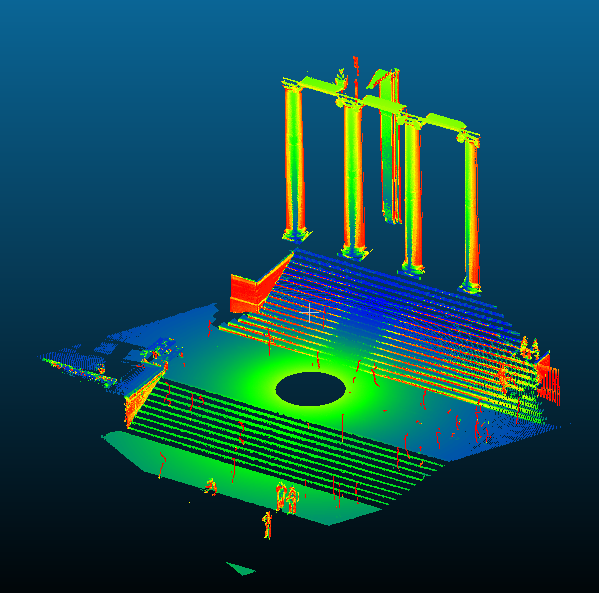
\includegraphics[width=0.8\linewidth]{./Anglek=60}
		\captionof{figure}{{\footnotesize Angle from
		vertical with $K = 60$}}
		\label{fig:Angleformvertk=60}
	\end{minipage}
	\end{minipage} %
	\begin{minipage}{.1 \textwidth}
		\begin{figure}[H]
			
			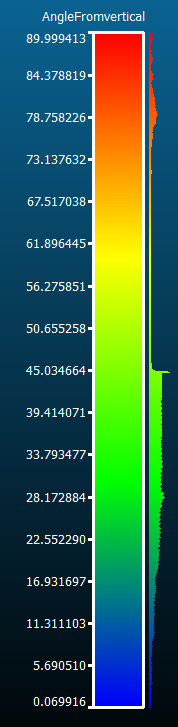
\includegraphics[width=1\linewidth]{./Lrdgend}
		\end{figure}

	\end{minipage}
	
	The above images show the angle from vertical for the three K values.
	\\
	It can be seen here that the best result is the K = 20. the classification of that image looks like this:
	\begin{figure}[H]
		\centering
		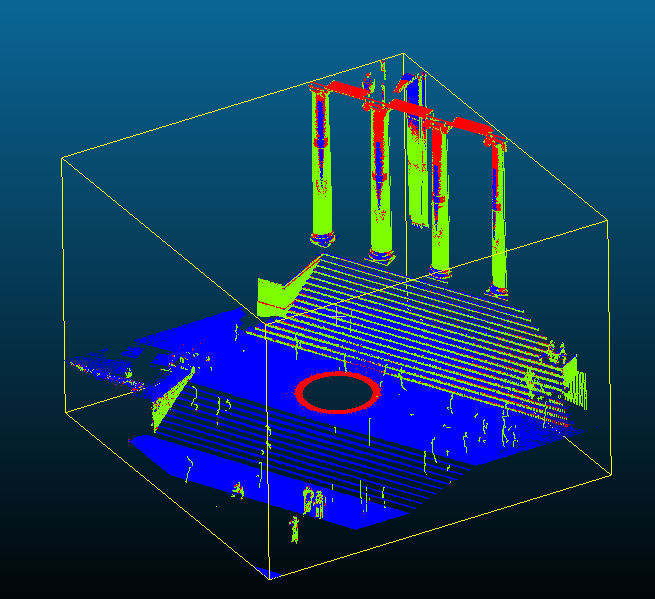
\includegraphics[width=0.4\linewidth]{./Classidfication2}
		\caption{Classification of scan with $K = 20$}
		\label{fig:Classidfication2}
	\end{figure}
	Where Blue is class 1, Red is class 2 and Green is class 3.

	\newpage
	\section{Additional Questions}

	\begin{description}
		 \item[1] Suggest how the program could be extended to perform a point cloud segmentation/classification.
		 
		 \item[] The program can classify a point cloud by grouping points with the same angle from vertical together.
		 
		 \item[2] Besides the angle to the vertical, what other features can we extract that could be used for a point cloud classification? 
		 		 
		 \item[] To extend a program like this to take more factors into the classification is not impossible. but it would take a complete rethink on the classification method, as opposed to looking at one factor you could look at the normal as well as other factors such as texture, intensity, colour, ect...
		 		 
		 These would then all need to be mapped into feature space and can be classified using already known classification algorithms like the Kmax method or the ISODATA method.

	\end{description}
	
	

	
\end{document}		